\section{Dot Product}
O Dot Product é o somatório da multiplicação entre dois vetores que vai resultar em um número real. Podemos entender o dot product como uma forma de fazer uma combinação linear entre dois vetores.

\vspace{0.5cm}

\begin{equation}
\begin{aligned}
    \mathbf{u}^T \times \mathbf{x} = [u_{\mathcolor{orange}{1}} u_{\mathcolor{orange}{2}} ... u_{\mathcolor{orange}{d}}]^T_{1 \times\mathcolor{orange}{D} }\times 
    \begin{bmatrix}
    x_{\mathcolor{orange}{0}} \\
    x_{\mathcolor{orange}{1}} \\
    \vdots \\
    x_{\mathcolor{orange}{d}}
\end{bmatrix}_{\mathcolor{orange}{D}\times 1} \quad \\
\end{aligned}
\end{equation}

\begin{equation*}
    = u_{\mathcolor{orange}{0}}x_{\mathcolor{orange}{0}} + u_{\mathcolor{orange}{1}}x_{\mathcolor{orange}{1}} + u_{\mathcolor{orange}{2}}x_{\mathcolor{orange}{2}} ... +u_{\mathcolor{orange}{d}}x_{\mathcolor{orange}{d}}
\end{equation*}

\begin{equation*}
= \sum_{i=1}^{d} u_{\mathcolor{orange}{i}}x_{\mathcolor{orange}{i}}
\end{equation*}

\vspace{0.5cm}

Propriedades importantes do dot product:
\begin{itemize}
    \item Comutativa: $\mathbf{u}^T \mathbf{x} = \mathbf{x}^T \mathbf{u}$
    \item Distributiva: $\mathbf{u}^T (\mathbf{x} + \mathbf{v}) = \mathbf{u}^T \mathbf{x} + \mathbf{u}^T \mathbf{v}$
\end{itemize}

\vspace{0.5cm}

Além dessa interpretação algébria, podemos interpretar o dot product de forma geométrica. Todo vetor tem as propriedades de magnitude e direção. A magnitude pode ser entendida como o tamanho do vetor, e a direção como o ângulo que o vetor faz com o eixo horizontal.

\begin{figure}[H]
    \centering
    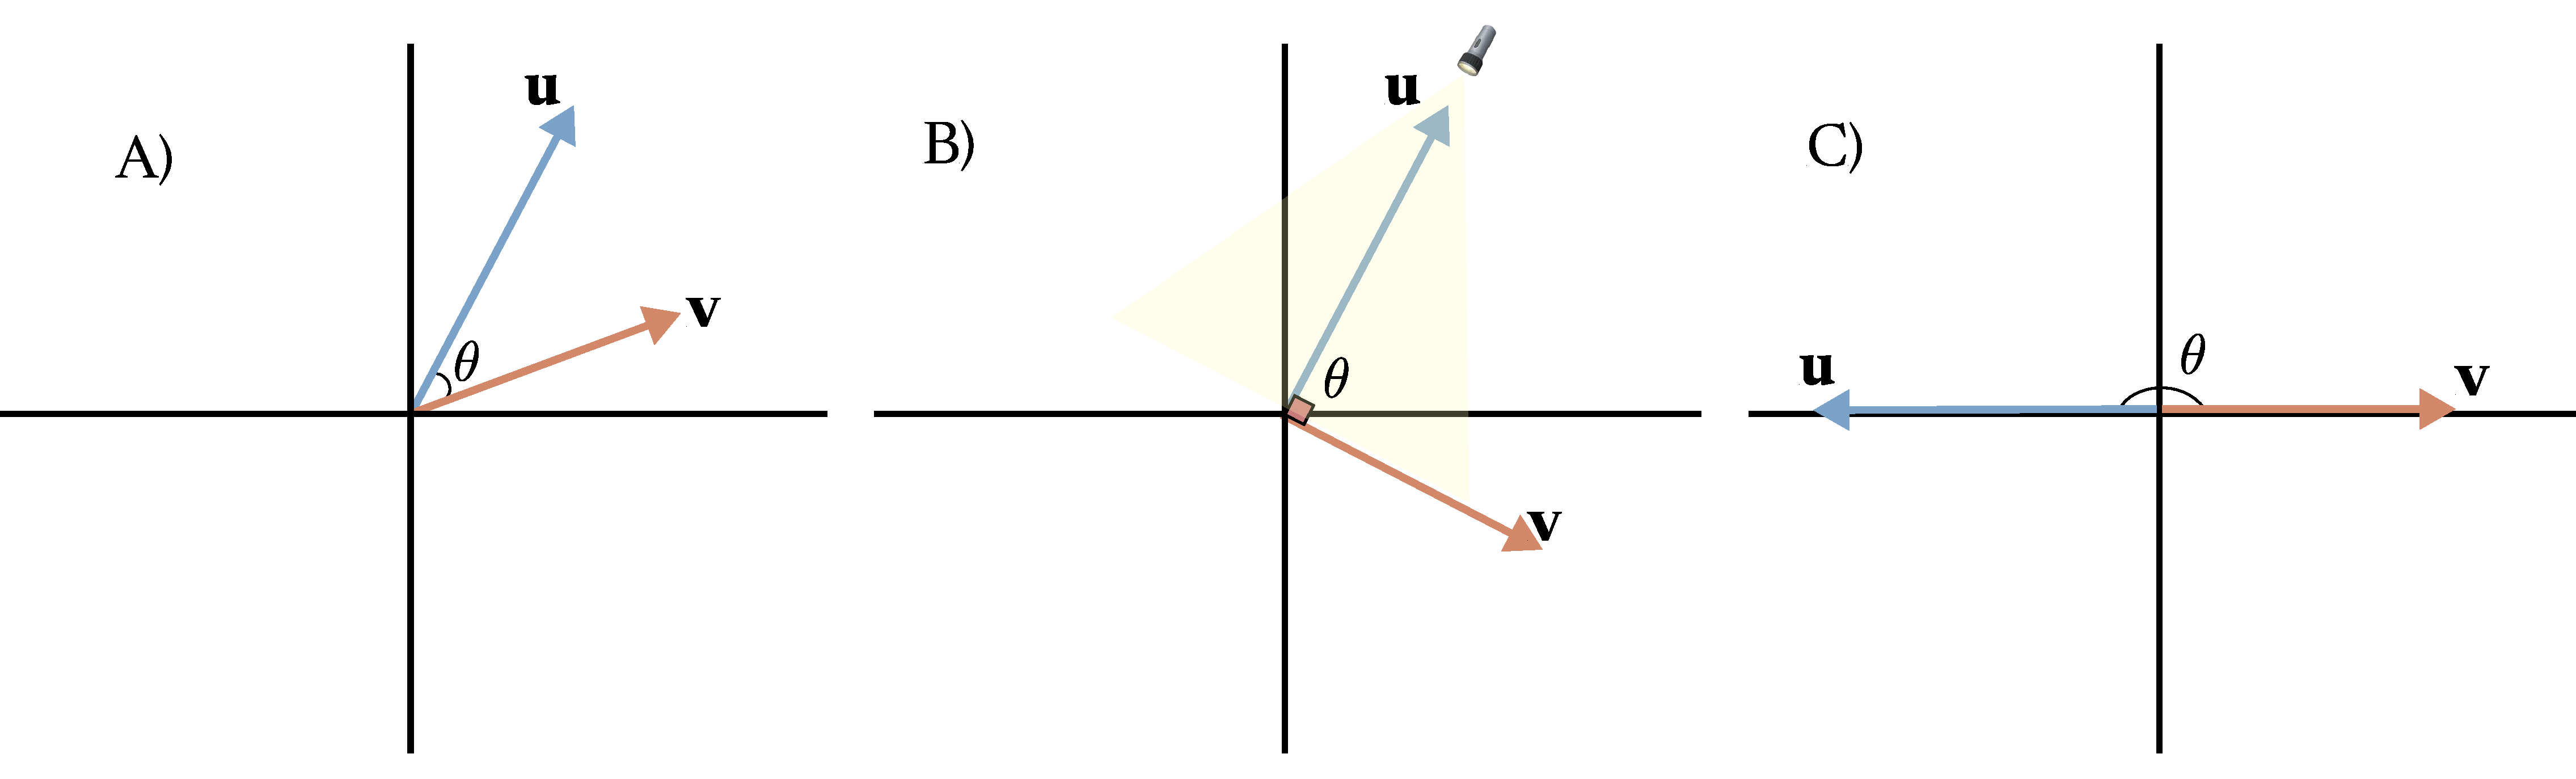
\includegraphics[width=1\linewidth]{Parts/MathematicalFoundations/Chapters/LinearAlgebra/Images/allDotProducts.pdf}
    \caption{}
    \label{fig:dot_product_geometry}
\end{figure}


 O dot product representa a multiplicação das magnitudes dos vetores e o cosseno do ângulo entre eles. 


\begin{equation*}
\mathbf{u} \cdot \mathbf{v} = |\mathbf{u}||\mathbf{v}|\cos(\theta)
\end{equation*}


% \begin{figure}[H]
%     \centering
%     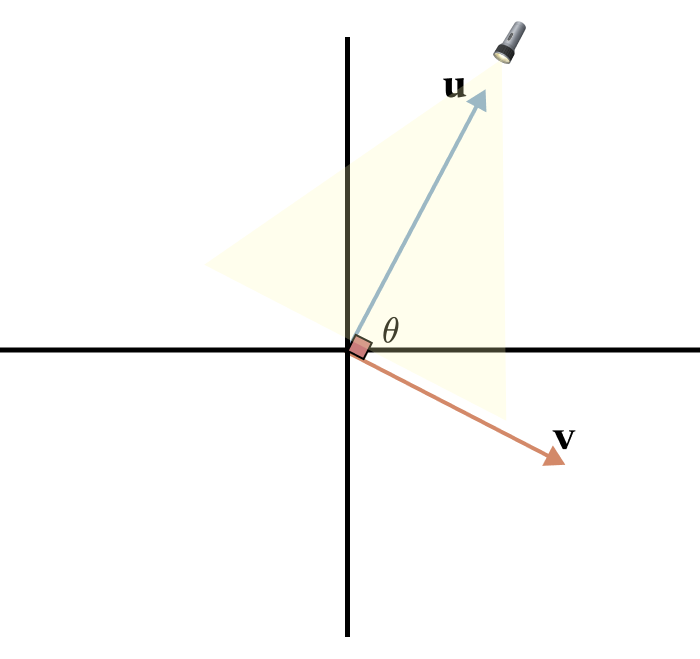
\includegraphics[width=0.5\linewidth]{Parts/MathematicalFoundations/Chapters/LinearAlgebra/Images/orthogonalVectors.png}
%     \caption{}
%     \label{fig:dot_product_geometry_orthogonalVectors}
% \end{figure}

Quando os vetores são otogonais, ou seja, formam um ângulo de 90 graus entre eles $\theta = 90^\circ$, o $\cos(\theta)$ será igual a zero. Esse cenário mostrado na \ref{fig:dot_product_geometry}-B descreve o caso onde a projeção de um vetor no outro é nula. Outro caso interessante é quando os vetores estão em direções opostas, ou seja, formam um ângulo de 180 graus entre eles $\theta = 180^\circ$. Nesse caso, o $\cos(\theta)$ será igual a -1, e o dot product resultará em um valor negativo. Esse cenário é ilustrado na \ref{fig:dot_product_geometry}-C, onde a projeção de um vetor no outro é negativa.

